\documentclass[12pt]{article}
\usepackage[margin=1in]{geometry}
\usepackage{setspace}
\usepackage{graphicx}
\onehalfspacing

\title{RCT Analysis: Impact of AI Tool on Loan Processing Clerks}
\author{Ilnaz Bagheri}
\date{April 2026}

\begin{document}
\maketitle

\section*{Interpretation}

This study evaluates the causal effect of an AI-assisted PDF extraction 
tool on worker productivity and quality using data from a randomized 
controlled trial conducted during March 2026 audit week. A total of 141 
loan processing clerks were observed, with 71 assigned to the treatment 
group (AI tool access) and 70 to the control group (manual entry).

The balance test confirmed successful randomization. Pre-treatment 
characteristics including years of experience (treated: 4.79, control: 
4.68, p=0.740), baseline tasks per hour (8.64 vs. 8.76, p=0.569), and 
training scores (87.77 vs. 87.09, p=0.481) showed no statistically 
significant differences between groups. This supports the ignorability 
assumption: treatment assignment was independent of pre-existing worker 
characteristics.

Regarding SUTVA, spillover effects are unlikely in this setting. Clerks 
processed loan applications independently, with no shared queues or 
collaborative workflows between treatment and control groups during the 
observation period.

The ATE estimates reveal a meaningful productivity gain. Treated clerks 
completed an average of 8.67 more tasks per shift than control clerks 
(p<0.0001), representing a substantial increase in throughput. However, 
the error rate also increased by 0.57 percentage points among treated 
workers (p=0.0002), suggesting a quantity-quality tradeoff. Workers 
using the AI tool processed more applications but introduced slightly 
more errors.

These findings have important implications for firms considering broad 
AI deployment. While the productivity gains are significant and 
economically meaningful, the increase in error rates warrants attention. 
Firms should consider pairing AI tools with quality control mechanisms 
to capture efficiency gains without sacrificing accuracy. A phased 
rollout with targeted training may help workers adapt to AI-assisted 
workflows while maintaining quality standards.

\begin{figure}[h]
\centering
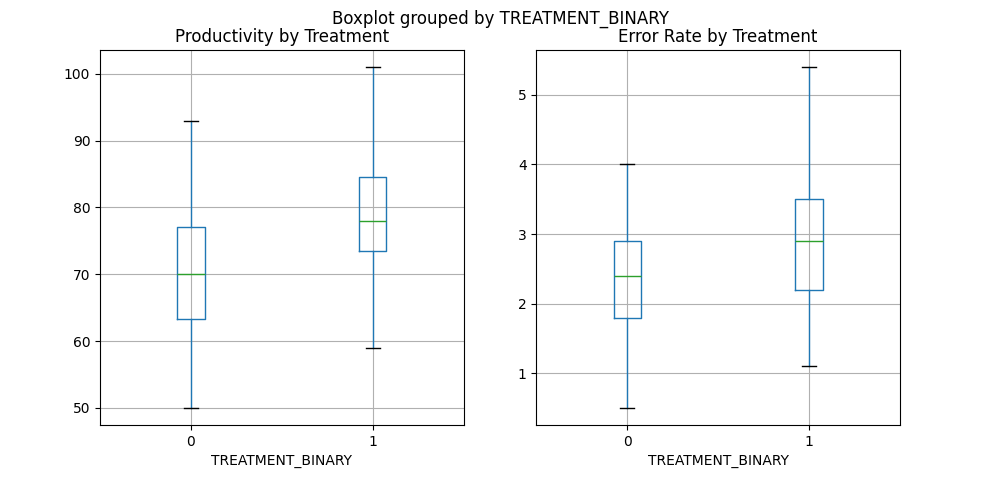
\includegraphics[width=0.9\textwidth]{boxplots.png}
\caption{Productivity and Error Rate by Treatment Group}
\end{figure}

\end{document}